\documentclass{article}
\usepackage{graphicx} % Required for inserting images

\title{Trabajo Práctico 1 - Teoría de Juegos}
\author{Juani Elosegui}
\date{Agosto 2024}

\begin{document}
    \maketitle

    \newpage
    
    \section{¿Verdadero o falso? Discuta las siguientes afirmaciones.}
        \subsection*{Respuestas}
            \begin{itemize}
                \item \textbf{Falso.} Recordemos que en los juegos de coordinación existen múltiples equilibrios de Nash, dado que los jugadores pueden tener intereses en común. Se puede demostrar un contraejemplo en el que existan dos equilibrios de Nash que tengan como pagos (A:2, B:2) y (A:1, B:1). Los dos pagos que representan un equilibrio de Nash para los jugadores A y B son válidos, no se eliminaría ninguna de estas dos estrategias porque ninguna es estrictamente dominante sobre otra, y para los jugadores existe más de una manera de coordinarse para que los pagos sean mutuamente beneficiosos.

                \item \textbf{Falso.} Pueden existir juegos en los cuales todas las estrategias posibles representan el mismo pago, es decir (a modo de ejemplo) que todas las estrategias pagan (1,1) a los jugadores A y B, respectivamente. En un escenario como este, no hay dominancia, por lo que todas las estrategias se podrían considerar racionalizables.
            \end{itemize}

    \section{Subastas}
        \subsection*{Respuestas}
            \textbf{a)}
                \begin{figure}[h]
                    \centering
                    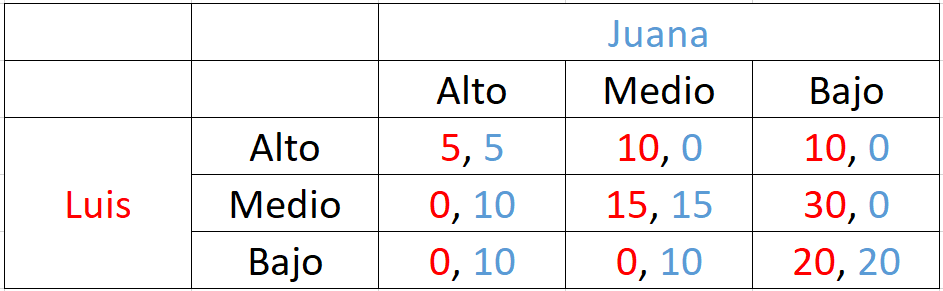
\includegraphics[width=0.5\linewidth]{fig1.png}
                \end{figure}\\
            \textbf{b)} La combinación (Bajo, Bajo) es un equilibrio de Nash, y también la combinación (Medio, Medio) porque, en esas situaciones, ninguno tiene incentivo para desviarse de su estrategia.
            \textbf{c)}
                \begin{figure}[h]
                    \centering
                    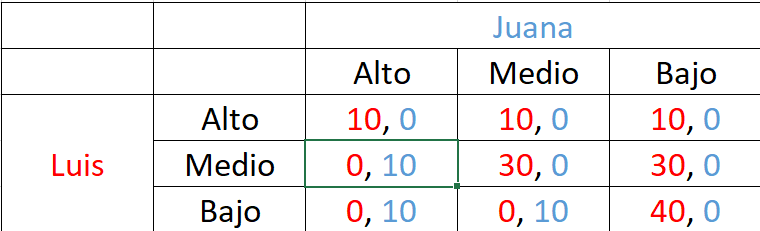
\includegraphics[width=0.5\linewidth]{fig2.png}
                \end{figure}\\
            \textbf{d)} No hay equilibrios de Nash en estrategias puras porque los dos van a querer cambiar su estrategia basándose en la estrategia tomada por el otro.\\
            \textbf{e)} En el formato 1 (subasta con empate) el pago esperado es:
                \[\frac{1}{9}\cdot (20+0+0+30+15+0+10+10+5) = \]
                \[\frac{1}{9}\cdot (20+30+15+10+10+5) = \]
                \[\frac{1}{9}\cdot 90 = \]
                \[10\]

            En el formato 2 (en caso de empate, gana Luis), el pago esperado es:
                \[\frac{1}{9}\cdot (40+0+0+30+30+0+10+10+10) = \]
                \[\frac{1}{9}\cdot (40+30+30+10+10+10) = \]
                \[\frac{1}{9}\cdot 130 = \]
                \[\frac{130}{9} = \]
                \[\approx 14\]

            El pago esperado para el vendedor de la obra es mayor si se implementa el formato 2. ($14 > 10$). Es evidente el porqué es conveniente usar este formato.

    \section{Estrategias continuas}
        \subsection*{Respuestas}
            \textbf{a)} Para hallar los equilibrios de Nash, tengo que derivar las funciones de utilidad de los dos amigos $s_{1}$ y $s_{2}$.

                Tenemos que:
                \[u_{1}(s_{1},s_{2}) = s_{1}+s_{2}+8+(8-s_{1})(s_{1}+s_{2})\]

                Simplifico, termina quedando:
                \[u_{1}(s_{1},s_{2}) = 8 + s_{2}(1+8-s_{1})+8s_{1}-s^{2}_{1}\]

                Derivo la función de utilidad con respecto a $s_{1}$:
                \[\frac{\partial u_{1}}{\partial s_{1}} = 8 - 2s_{1} + s_{2}-s_{2}\]
                \[\frac{\partial u_{1}}{\partial s_{1}} = 8 - 2s_{1}\]

                Igualo a 0 para encontrar el equilibrio:
                \[\frac{\partial u_{1}}{\partial s_{1}} = 0\]
                \[8 - 2s_{1} = 0\]
                \[s_{1} = 4\]

                Si repito el mismo proceso para $u_{2}(s_{1},s_{2})$, terminaría quedando que el equilibrio para $s_{2}$ es:
                \[s_2 = 4\]

                Finalmente, el equilibrio de Nash es $s_{1} = 4, s_{2} = 4$.\\

            \textbf{b)} En el inciso a) encontré el equilibrio de Nash de los dos amigos. En este equilibrio, los dos deciden limpiar 4hs cada uno. Si alguno quisiera limpiar más y otro menos, o bien los dos quisieran limpiar más o menos del equilibrio encontrado, la utilidad disminuiría, ya que van a ver menos televisión y el departamento puede seguir estando sucio.

            Esto se relaciona con el Dilema del Prisionero, porque como beneficia a los dos limpiar, los incentivos individuales de cada uno puede hacer que limpien menos horas llevaría a una situación de utilidad no tan óptima como la del equilibrio.

    \section{Búsqueda de equilibrios}
        \subsection*{Respuestas}
            \textbf{a)} No existe un equilibrio en estrategias estrictamente dominantes porque solo uno de los jugadores tiene una estrategia estrictamente dominante ('C' para el Jugador 1), pero el otro no tiene una estrategia estrictamente dominante.\\
            \textbf{b)} Por otro lado, sí existe un equilibrio bajo el concepto de eliminación iterativa de estrategias estrictamente dominadas, que es cuando el Jugador 1 juega 'A' y el Jugador 2 juega 'a'.
        
\end{document}
